\chapter{評価実験}

\label{chap:evaluation}

\section{実験環境}
	\subsection{データセット生成}
		感性語の抽出を行うにあたり,感情表現辞典に掲載された情報を活用する.
		感情表現辞典に収録されている単語と熟語の合計2278語のうち,
		MeCabで分かち書きを行うことで複数単語に別れてしまうものを除くと,
		1245語となる.
		本実験におけるデータセット生成では,これらを感性語とする.

		データセット生成のためのテキストデータには
		Wikipediaのテキストに前処理を施した状態で公開されている
		Wiki-40Bデータセットの日本語版を用いる.
		1文ずつに分割したとき,Wiki-40Bデータセットに含まれる文章の数は,
		$Train/Val/Test=12,330,278/677,757/678,490$となった.
		これらのうち,感性語を含む文は
		$Train/Val/Test=2,337,909/128,126/128,698$となった.
		本実験では,ウィンドウサイズ$W=3$とし,感性語の周辺単語を収集した.
		このBERTが出力した分散表現と感情ベクトルがペアになった
		データセットのサイズは,
		$Train/Val/Test=20,154,529/1,104,904/1,108,482$
		となった.

	\subsection{ニューラルネットワークの学習条件}
		入力が768次元の単語分散表現で,出力が10次元の感情ベクトルとなる.
		本実験では図\ref{fig:network}で示すような,中間層を400次元とした
		非常にシンプルな3層のニューラルネットワークを構築し,
		生成したデータセットを用いて学習を行った.
		\begin{figure}[H]
			\centering
			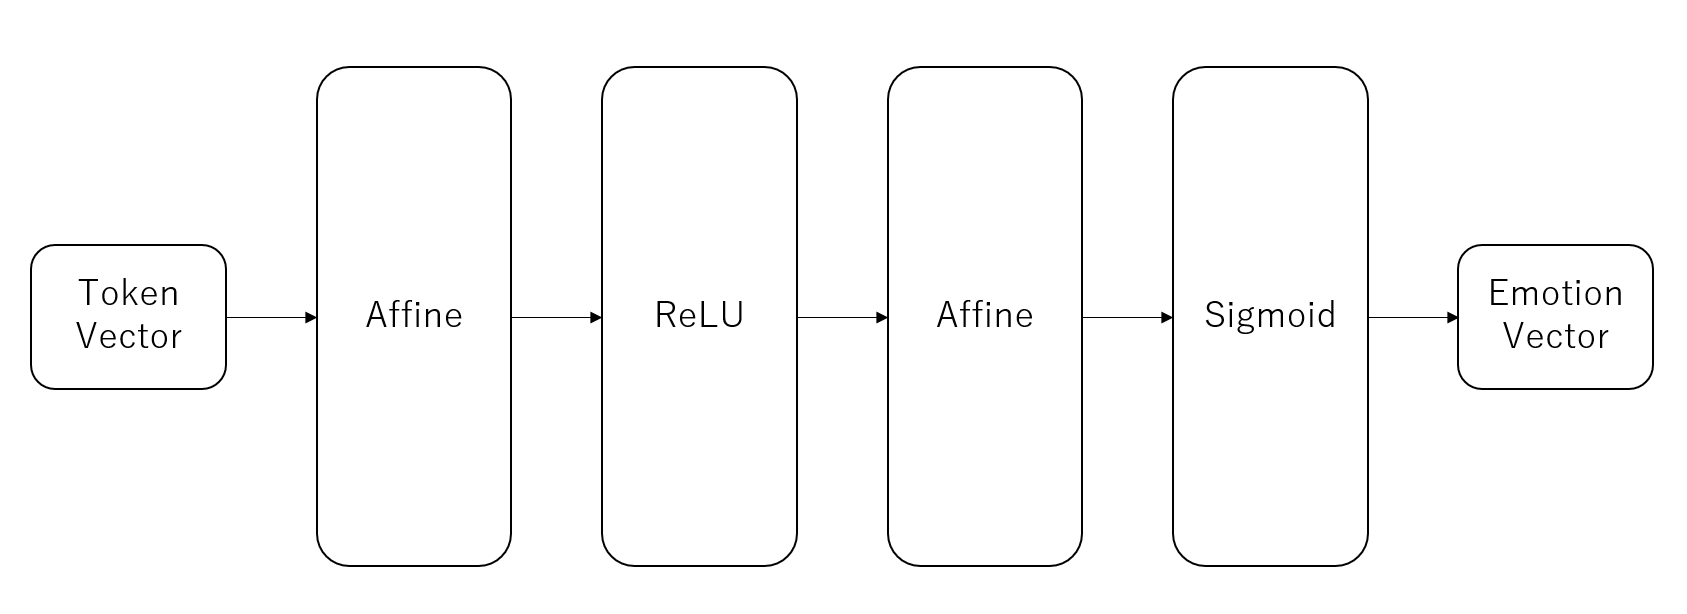
\includegraphics[width=\linewidth]{./figure/network.png}
			\caption{ニューラルネットワークの構造}
			\label{fig:network}
		\end{figure}
		中間層の活性化関数はReLU関数とし,
		出力層にsigmoid層を通すことにより,0以上1以下の値に変換する.
		sigmoid関数は以下の式で示される.
		\begin{equation}
			f(x)=\frac{1}{1+e^{-x}}
		\end{equation}
		この時,出力された10次元のベクトルが,データセットに与えられた
		感情ベクトルに近づくよう学習を行うことになる.
		損失関数は最小二乗誤差とし,Adamにより学習率$1\times10^{-3}$で最適化を行った.
		エポック数については,Early Stoppingで5回以上validation lossが更新
		されなかった段階で学習を終了させた.
		
	\subsection{比較手法}
		本手法と比較するためのベースライン手法として,BERT Layerを通す前の
		Embedding Layerによる分散表現をネットワークの入力とした場合を設定する.
		BERT Layerを通すことにより,Transformerによる周りの単語の影響を加味することになる.
		今回設定したベースラインではEmbedding Layerによる
		分散表現を利用することで周辺単語の影響が含まれないことになる.
		また、感性語の周辺単語に与える感情ベクトルについて
		距離に応じた重み付けを行うことによる効果を確認するため,
		重み付けを行うBERT+weight,行わないBERTに分けて実験を行う.

\section{感情ベクトルの生成例}
	入力文に対する各単語の感情ベクトル出力例を以下に示す.
	\subsection{「仕事は人生を豊かにしてくれる.」に対する出力}
		\begin{figure}[H]
			\begin{tabular}{cc}
				\begin{minipage}[t]{0.45\hsize}
					\centering
					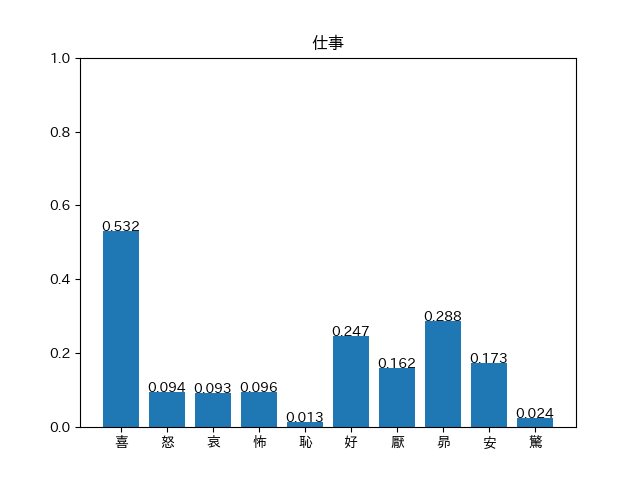
\includegraphics[keepaspectratio, scale=0.45]{./figure/output/Q01/001.png}
					\subcaption{「仕事」に対する感情ベクトル}
				\end{minipage} &
				\begin{minipage}[t]{0.45\hsize}
					\centering
					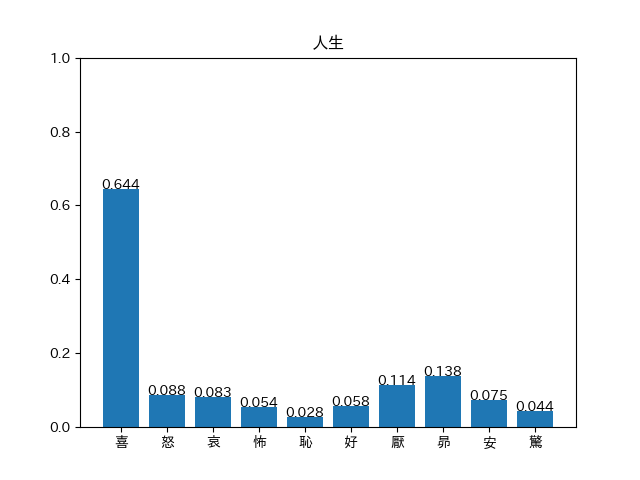
\includegraphics[keepaspectratio, scale=0.45]{./figure/output/Q01/002.png}
					\subcaption{「人生」に対する感情ベクトル}
				\end{minipage} \\
				\begin{minipage}[t]{0.45\hsize}
					\centering
					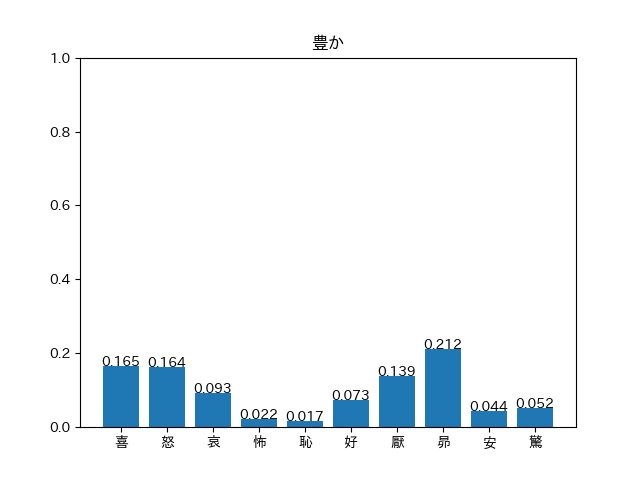
\includegraphics[keepaspectratio, scale=0.45]{./figure/output/Q01/003.png}
					\subcaption{「豊か」に対する感情ベクトル}
				\end{minipage} &
				\begin{minipage}[t]{0.45\hsize}
					\centering
					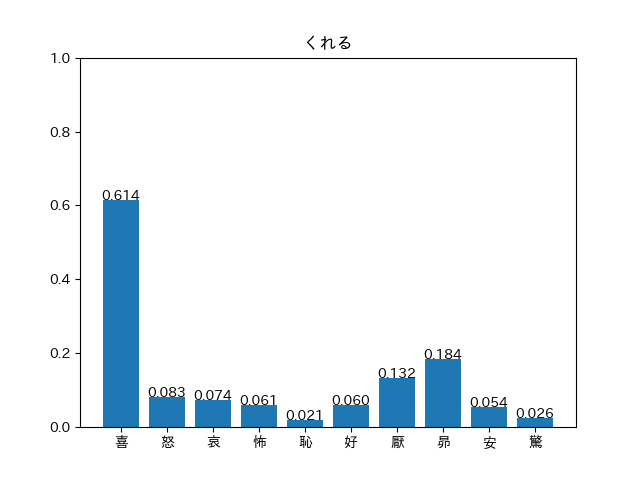
\includegraphics[keepaspectratio, scale=0.45]{./figure/output/Q01/004.png}
					\subcaption{「くれる」に対する感情ベクトル}
				\end{minipage} \\
			\end{tabular}
			\caption{「仕事は人生を豊かにしてくれる.」に対する各単語の感情ベクトル}
			\label{fig:output_ex01}
		\end{figure}

		\subsection{「仕事は面倒だし、疲れるから嫌だ。」に対する出力}
		\begin{figure}[H]
			\begin{tabular}{cc}
				\begin{minipage}[t]{0.45\hsize}
					\centering
					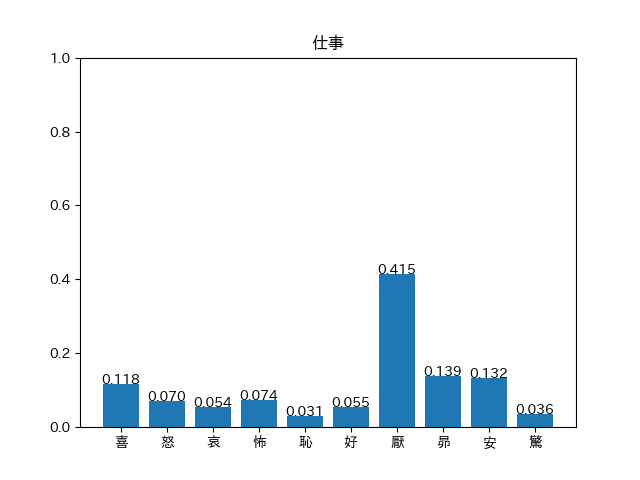
\includegraphics[keepaspectratio, scale=0.45]{./figure/output/Q02/001.png}
					\subcaption{「仕事」に対する感情ベクトル}
				\end{minipage} &
				\begin{minipage}[t]{0.45\hsize}
					\centering
					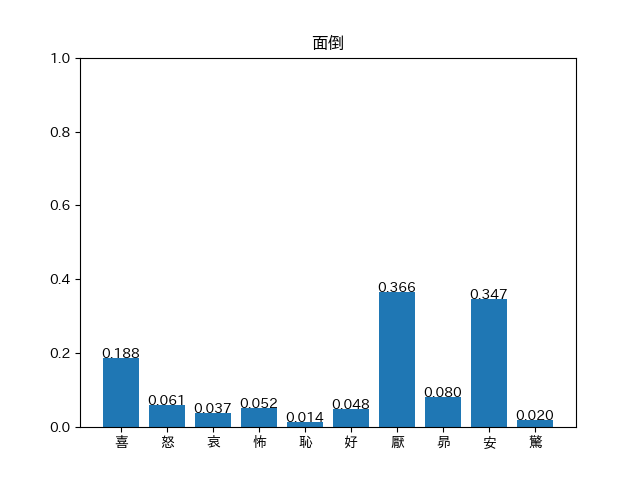
\includegraphics[keepaspectratio, scale=0.45]{./figure/output/Q02/002.png}
					\subcaption{「面倒」に対する感情ベクトル}
				\end{minipage} \\
				\begin{minipage}[t]{0.45\hsize}
					\centering
					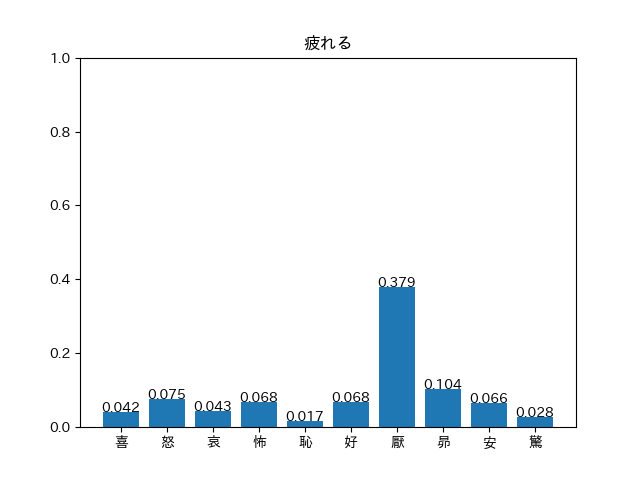
\includegraphics[keepaspectratio, scale=0.45]{./figure/output/Q02/003.png}
					\subcaption{「疲れる」に対する感情ベクトル}
				\end{minipage} &
				\begin{minipage}[t]{0.45\hsize}
					\centering
					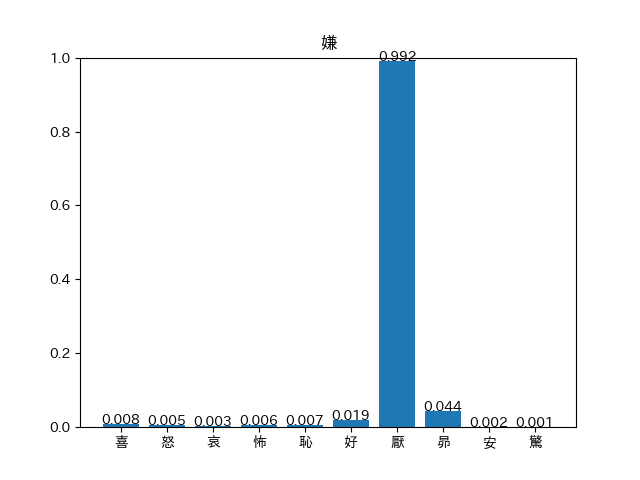
\includegraphics[keepaspectratio, scale=0.45]{./figure/output/Q02/004.png}
					\subcaption{「嫌」に対する感情ベクトル}
				\end{minipage} \\
			\end{tabular}
			\caption{「仕事は面倒だし、疲れるから嫌だ.」に対する各単語の感情ベクトル}
			\label{fig:output_ex02}
		\end{figure}

		図\ref{fig:output_ex01}ではポジティブな文脈で「仕事」という単語を用いているのに対し,
		図\ref{fig:output_ex02}ではネガティブな文脈で「仕事」という単語を用いている.
		それぞれの「仕事」に対する感情ベクトルを比較すると,
		文脈に応じてその出力が変化していることがわかる.

\section{単語の感情推定の妥当性に関する評価実験}
	\subsection{実験設定}
		本実験では,本システムにより出力された単語の感情ベクトルが
		人間の想起する感情のイメージと合致しているのかを検証する.
		実験に先立ち,被験者には特定の単語を用いるような文章を生成してもらい,
		システムに入力したうえで,文章生成時に指定した単語(以下,対象単語とよぶ)
		の感情ベクトルを出力した.
		対象単語について,それが用いられた文脈を考慮した上で想起されるような
		感情を感情ベクトルの形で被験者に予想してもらった.
		システム出力,被験者により予想された感情ベクトルをそれぞれ正規化したうえで,
		Top-1精度,Top-3精度,コサイン類似度を比較する.
		同次元のベクトル$\bold{a},\bold{b}$について,これらのコサイン類似度は
		以下のように計算される.
		\begin{equation}
			cos(\boldsymbol{a},\boldsymbol{b})=\frac{\boldsymbol{a}\cdot\boldsymbol{b}}{\|\boldsymbol{a}\|\|\boldsymbol{b}\|}
		\end{equation}

	\subsection{実験結果}
		\begin{table}[H]
			\centering
			\caption{実験1の結果}
			\label{table:top-k_cos-sim_all}
				\begin{tabular}{cccc}
					\hline
					& Top-1 & Top-3 & cos類似度 \\
					\hline \hline
					BERT+weight & 32.95\% & 61.36\% & \textbf{0.612} \\
					BERT & \textbf{37.50}\% & \textbf{65.91}\% & 0.609 \\
					embedding & 26.14\% & 53.41\% & 0.557\\
					\hline
				\end{tabular}
		\end{table}
	\subsection{考察}
		これから分析を行います.
		\begin{itemize}
			\item Top-k精度では,感性語との距離に応じて付与するベクトル強度に重み付けを行ったBERT+weightよりも,重み付けを行っていないBERTのほうが高性能.
			\item cos類似度ではBERT+weightが最高性能
		\end{itemize}
		これらの結果から,最も強く想起する感情を判定すると,
		強度の高いベクトルを与えたBERTのほうが,強度を弱めているBERT+weightよりも高性能が出る.
		しかし,ベクトル全体の距離をcos類似度で測ると,BERT+weightが高性能であることから,
		複数の感情が想起されるケースなどではBERT+weightのほうがより良い出力を行っている可能性がある.
		
		このような流れでまとめていこうと考えています.
		\begin{table}[H]
			\centering
			\caption{単語の種類別で分けた実験1のTop-k精度}
			\label{table:top-k_cos-sim_hinshi}
				\begin{tabular}{ccccccc}
					\hline
					& \multicolumn{3}{c}{\textbf{Top-1}} & \multicolumn{3}{c}{\textbf{Top-3}} \\
					& 一般単語 & 感性語 & 感性多義語 & 一般単語 & 感性語 & 感性多義語 \\
					\hline \hline
					BERT+weight & \textbf{27.78}\% & \textbf{61.11}\% & 23.53\% & \textbf{58.33}\% & \textbf{77.78}\% & 55.88\% \\
					BERT & 25.00\% & \textbf{61.11}\% & \textbf{38.24}\% & \textbf{58.33}\% & \textbf{77.78}\% & \textbf{67.65}\% \\
					embedding & 11.11\% & 50.00\% & 29.41\% & 33.33\% & 72.22\% & 64.71\% \\
				\hline
				\end{tabular}
		\end{table}

		単語の種類別で精度を出した時の特徴についてもまとめていこうと考えています.

					

\section{一般単語感情推定の文脈考慮性に関する評価実験}
	\subsection{実験設定}
		本実験では,同一の単語に対する出力がその出現する文脈に応じて
		適切に変化するのかを検証する.
		特定の単語(以下,対象単語と呼ぶ)を含み,文脈がポジティブ・ネガティブになるような文章を
		それぞれ被験者に生成してもらい,システムに入力した.
		本手法により得られた対象単語の感情ベクトルについて,
		それぞれの出力で,適切な感情を出力できているか,
		不適切な感情の出力を抑制できているかを,
		また対象単語について,用いられる文脈が異なっている
		2つの出力を比較して,文脈を考慮した出力になっているかを
		それぞれ1(最低)~5(最高)の5段階評価で評価してもらった.


	\subsection{実験結果}
	\begin{table}[H]
		\centering
		\caption{実験2の結果}
		\label{normal_word_result}
			\begin{tabular}{cccc}
				\hline
				& 適切な感情の出力 & 不適切な感情の出力の抑制 & 文脈考慮性 \\
				\hline \hline
				BERT+weight & 3.93 & \textbf{3.82} & \textbf{3.92} \\
				BERT & \textbf{3.98} & 3.76 & 3.91 \\
				embedding & 3.22 & 2.88 & 2.60 \\
				\hline
			\end{tabular}
		\end{table}
	\subsection{考察}
	これから分析を行います.
	\begin{itemize}
		\item 適切な感情の出力でBERTが最高性能,不適切な感情の抑制と文脈考慮性でBERT+weightが高性能
	\end{itemize}
	このことから,周辺単語について距離を弱めるBERT+weightのほうが,
	不適切な感情を抑えることができている可能性があると考えています.

\section{感性多義語感情推定の文脈考慮性に関する評価実験}
	\subsection{実験設定}
	本実験では,データセット生成に用いた感情表現辞典において,
	多くの感情を想起するとされている,多義性のある感性語(以下,感性多義語とよぶ)
	に対しても,文脈を考慮して適切な感情を出力することができるのか
	を検証する.
	本実験では,4つ以上の感情を想起するとされていた感性多義語の中から,
	「気持ち」,「涙」,「思い」の3単語について,
	文脈考慮性を持った単語感情推定ができるのかを検証する.
	特定の感性多義語(以下,対象単語とよぶ)を含み,文脈が異なっている文章を
	あらかじめ被験者に生成してもらい,システムに入力した.
	本手法により得られた対象単語の感情ベクトルについて,
	それぞれの出力で適切な感情を出力できているか,
	不適切な感情の出力を抑制できているか,
	をそれぞれ1(最低)~5(最高)の5段階評価で評価してもらった.
	

	\subsection{実験結果}
	\begin{table}[H]
		\centering
		\caption{実験3の結果}
		\label{kansei_tagigo_result}
			\begin{tabular}{ccc}
				\hline
				& 適切な感情の出力 & 不適切な感情の出力の抑制 \\
				\hline \hline
				BERT+weight & 4.05 & \textbf{3.84} \\
				BERT & \textbf{4.12} & 3.48 \\
				embedding & 3.66 & 3.31 \\
				\hline
			\end{tabular}
	\end{table}

	\subsection{考察}
	これから分析を行います.
	\begin{itemize}
		\item 適切な感情の出力ではBERTが,不適切な出力の抑制ではBERT+weightが高性能と,一般単語同様の傾向が見られる.
	\end{itemize}
	このことから,一般単語の場合と同様の形でまとめる予定です.
